\chapter{UI Prototypes}\label{UI Prototypes}

\section{Prototype 1}

\begin{longtable}{@{}cc@{}}
    \caption{UI Prototypes for the Application}\label{fig:ui_prototypes} \\
    \centering
    \begin{subfigure}{.5\textwidth}
        \centering
        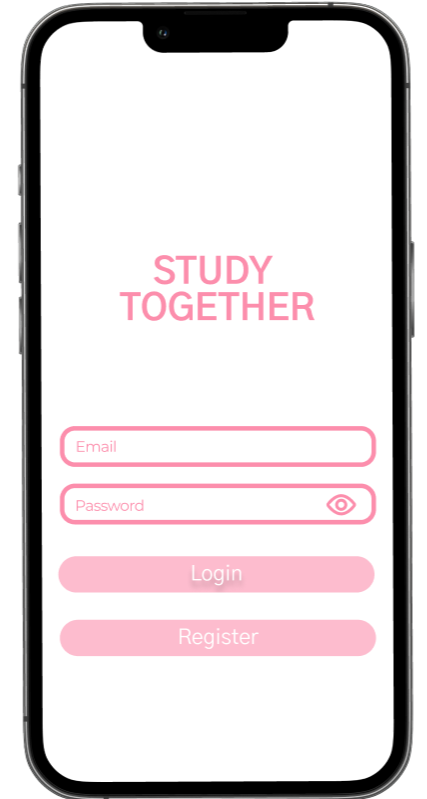
\includegraphics[width=.8\linewidth]{Figures/landing.png}
        \caption{\footnotesize Landing Page}
        \label{fig:landing}
    \end{subfigure}%
    &
    \begin{subfigure}{.5\textwidth}
        \centering
        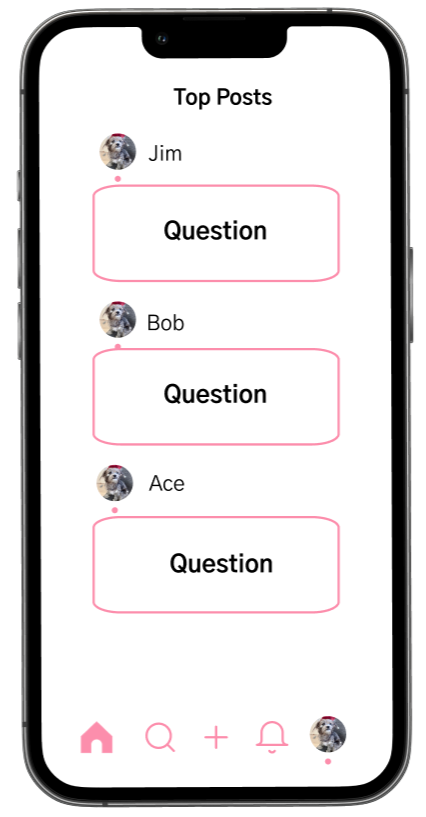
\includegraphics[width=.8\linewidth]{Figures/home.png}
        \caption{\footnotesize Home Page}
        \label{fig:home}
    \end{subfigure} \\
    
    \begin{subfigure}{.5\textwidth}
        \centering
        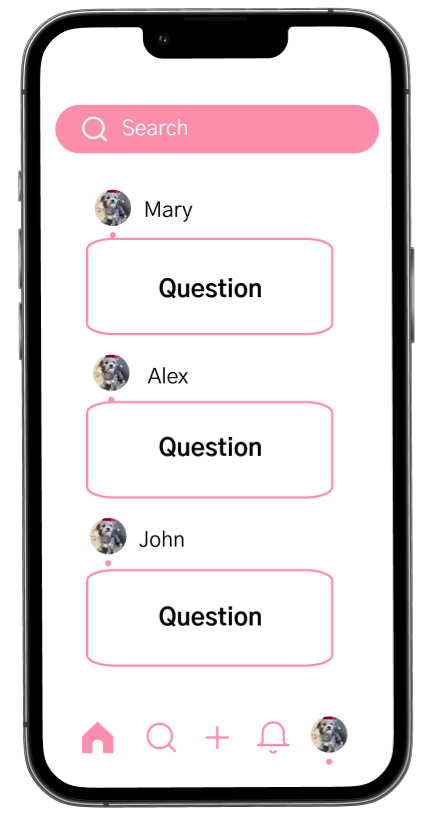
\includegraphics[width=.8\linewidth]{Figures/search.png}
        \caption{\footnotesize Search Page}
        \label{fig:search}
    \end{subfigure}%
    &
    \begin{subfigure}{.5\textwidth}
        \centering
        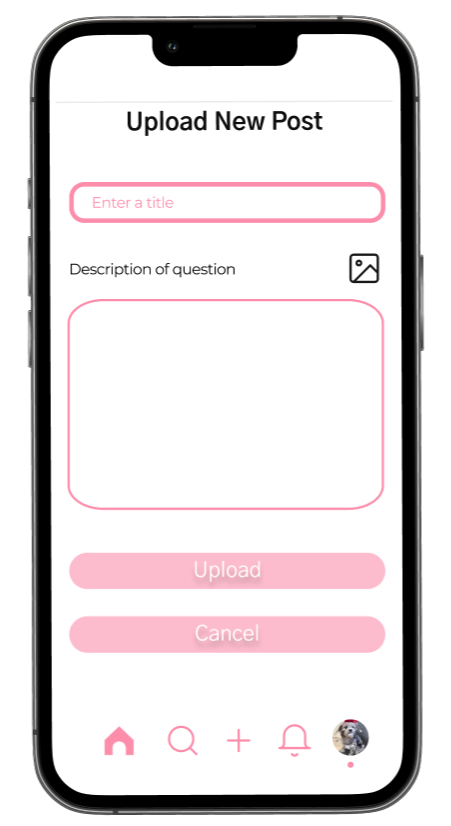
\includegraphics[width=.8\linewidth]{Figures/upload.png}
        \caption{\footnotesize Upload Page}
        \label{fig:upload}
    \end{subfigure} \\
    
    \begin{subfigure}{.5\textwidth}
        \centering
        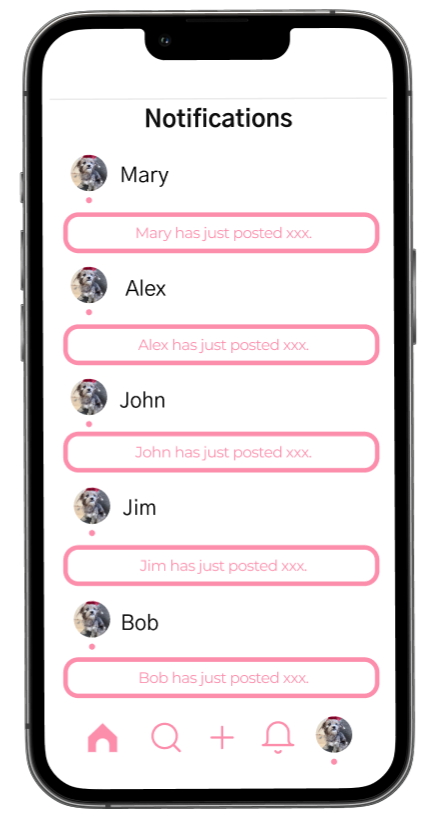
\includegraphics[width=.8\linewidth]{Figures/notification.png}
        \caption{\footnotesize Notification Page}
        \label{fig:notification}
    \end{subfigure}%
    &
    \begin{subfigure}{.5\textwidth}
        \centering
        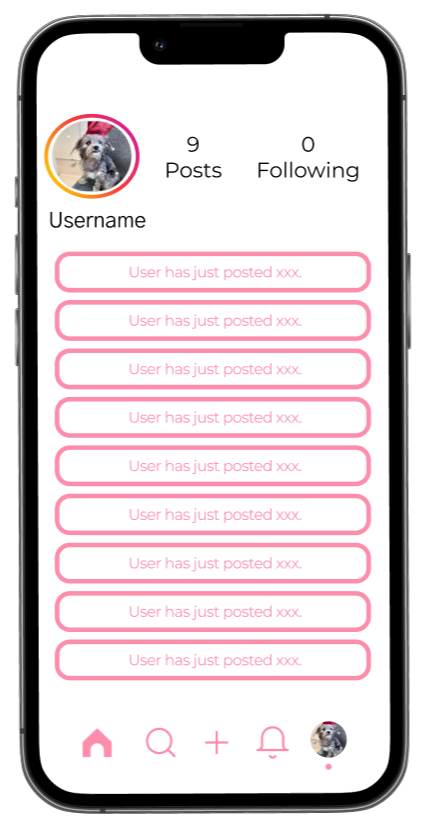
\includegraphics[width=.8\linewidth]{Figures/profile.png}
        \caption{\footnotesize Profile Page}
        \label{fig:profile}
    \end{subfigure} \\
\end{longtable}